%%% maw.tex
%% \section{Minimal Absent Words and Maximal Repeats}
\section{Minimal Rare Words and Maximal Repeats}
\label{sec:mrep}

We introduce a fundamental concept of maximal repeats of a string $S$, which is useful for realizing efficient enumeration of many kinds of unusual words. Then, we give a characterization of the set $\MAW(S)$ of minimal absent words of a string $S$. 
Let $S = S[1..n] \in \Sigma^n$ be a string over alphabet $\Sigma$ and $\hat S[0..n+1] = \# S\daller \in \hat\Sigma^{n+2}$ be its extended version with endmarkers.

%%%% 
\mysubsubsection{Maximal repeats}
%%%%
A repeat of $S$ is any substring $u \in \Sigma^+$ that occurs at least twice in $S$, that is, $u \in \Fac(S)$.
Let $u \in \Sigma+$ be any factor of $\hat S$. Since $\#, \daller \not\in \Sigma$, we see $u \in \Fac(S)$, namely, $u$ is contained in the content $S$.
%%% 
%% \begin{definition}[maximal repeat]\rm 
A string $u \in \Sigma+$ is a \textit{maximal repeat} of $S$ if it satisfies the following conditions: 
\begin{enumerate*}[(1)]
\item $u$ is a factor of $S$, i.e., $u \in \Fac(S)$;  
\item there exist two start positions $p, q \in \Spos[S](u)\;(p\not= q)$ of $u$ such that
  \begin{enumerate*}[(i)]
  \item $u$ is \textit{left-branching} meaning that the preceding characters are mutually different, i.e., $S[p-1] \not= S[q-1]$, and
  \item $u$ is \textit{right-branching} meaning that the following characters are mutually different, i.e., $S[p+|u|] \not= S[q+|u|]$. 
  \end{enumerate*}
\end{enumerate*}
%% \end{definition}
In what follows, $\MR(S)$ denotes the set of all maximal repeats of a string $S$. By definition, any $w$ in $\MR(S)$ correctly occurs at least twice in $S$. 

For later use, we define the \textit{set of left characters} $\LSigma(u) \subseteq \Sigma\cup\set{\#}$ (resp.~\textit{right characters} $\RSigma[](u) \subseteq \Sigma\cup\set{\daller}$) of a factor $u \in \Fac(S)$ to be the sets of all characters $S[p-1] \in \hat\Sigma$ (resp.~$S[p+|u|] \in \hat\Sigma$) preceding (resp.~following) all positions $p\in \Spos(u)$ of $u$ in $\hat S$.
If it is clear from context, we write $\LSigma[](u)$ and $\RSigma[](u)$ by omitting subscript $\hat S$. 
Using this notation, we can redefine a maximal repeat of $S$ to be any nonempty string $u \in \Fac(S)$ with $|\LSigma(u)| \ge 2$ and $|\RSigma(u)| \ge 2$.


\mysubsubsection[]{Minimal absent words}
%%%% 
A \textit{minimal absent word} (MAW) of a string $S$ are a class of unusual words, introduced by Garcia, Pinho, Rodrigues, Bastos, and Ferreira~\cite{garcia2011minimal}. A \textit{MAW} is a non-trivial string $w$ that does not occur in $S$, and any proper factor of $w$ occurs in $S$ as a substring (see \cite{garcia2011minimal}).
Precisely, a MAW of $S$ is a string $a u b$ with $a, b\in \hat\Sigma$ and $u \in \Sigma^+$ such that
\begin{enumerate*}[(i)]
\item $w \not\in \Fac(\hat S)$; and 
\item $au, ub \in \Fac(\hat S)$. 
\end{enumerate*}

As an example, the minimal absent words of the string $S = \texttt{aabaababb}$ are shown in \cref{fig:example:maw}. 

%%%%%%
%% \begin{algorithm}[t]
%% \centering  
%% %% 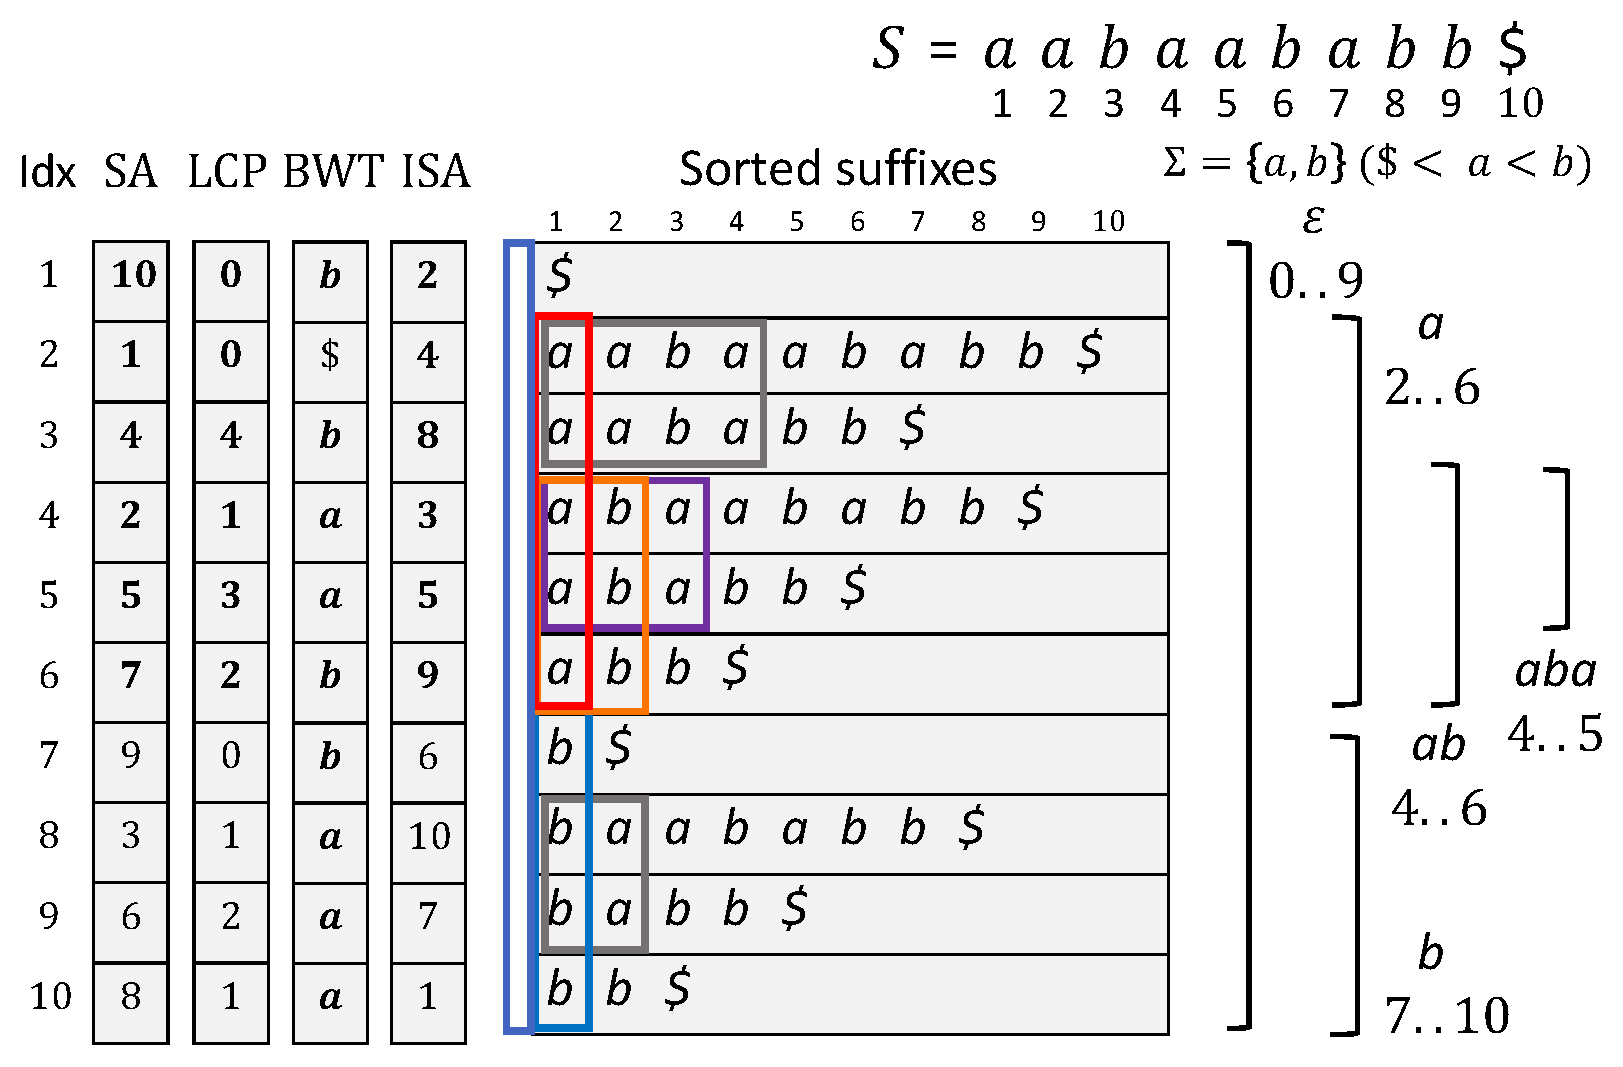
\includegraphics[width=0.60\textwidth]{fig/exp1/fig1.pdf}
%% \vspace{.5\baselineskip}
  %% \setlength{\interspacetitleruled}{0pt}%
%% \setlength{\algotitleheightrule}{0pt}%

\begin{algorithm}[t]
  \caption{A basic algorithm that, given a string $S[1..n]$ of length $n$ over alphabet $\Sigma = \set{0, \dots, \sigma-1}$, enumerates all maximal repeats of $S$ within the set $\MR(S)\cap \Theta$ that satisfy a monotone constraint $\Theta$ on $\MAW(S)$. Examples of monontone constraints are
    $\Theta_\idrm{maxlen} = \Sigma^{\le \ell}$ and 
    $\Theta_\idrm{minfreq} = \sete{ u \in \Sigma^*\mid \Occ(u) \ge s }$ for integers $\ell, s\ge 0$.
}\label{fig:example:maw:main}
\KwNotes{$S$ must satisfies $|\Sigma(S)| \ge 2$; Otherwise, start the procedure with as $root$ the triple for the shortest maximal repeat $\rext{\eps}$ in $S$.
}
\textbf{procedure} \MREnum$(\pair{i..j, \ell}, \Theta, Words)$\;
\Begin{
    Preprocess $\SA, \ISA, \LCP$ from a string $S$\;
    \While (\comblk{Runtime}) {a new request $\Theta$ is given by a user}{
      $Words \gets \emptyset$; 
      $root \gets \pair{1..n, 0}$\; 
      $Words \gets \MRRec(\pair{1..n, 0}, \Theta, Words)$\;
      Output $Words$\; 
    }
  }
\end{algorithm}

\begin{algorithm}[t]
  \caption{A subprocedure $\MRRec$ for enumerating all maximal repeats. See \cref{fig:example:maw:main} for its input and output.
}\label{fig:example:maw:sub}
%% \caption{Top-down MR-enumeration algorithm with \SA}\label{algo:maxrep:tdfw}
%% \KwInput{a string $S[1..n]$ of length $n$ over alphabet $\Sigma = \set{0, \dots, \sigma-1}$. }
%%%\medskip
%%  
  %% \KwInput{
  %%   A rich representation $\pair{i..j, \ell}$ for a factor of $S$,
  %%   and a set $Words$ of rich representations over $\pair{\SA, S}$. 
  %% }
  \KwInput{
    A triple $\pair{i..j, \ell} \in \RREP$,
    a constraint $\Theta \subseteq \Sigma^*$, and 
    a set $Words \subseteq \RREP$. 
  }
  \KwOutput{
    the set $\MR(S)$ of all maximal reepeats of the string $S$ prefixed by the word $u := \getfactor(i..j, \ell)$. 
  }
  \textbf{procedure} \MRRec$(\pair{i..j, \ell}, \Theta, Words)$\;
  \Begin{
      %\textbf{output} $(i..j, \ell)$
      \If{$u := \getfactor(i..j, \ell) \not\in \Theta$}{
        \Return $Words$\; 
      }
      $Words.\append(\pair{i..j, \ell})$
      \Comment*{A maximal repeat is found}
      $Children \gets \emptyset$\; 
      $Children \gets \GenChildren(i..j, \ell, Children)$\Comment*{See \cref{lem:genchildren}}
      \For %(\CM{})
           {each child $(c, \pair{i_c..j_c, \ell_c}) \in Children$}{
             \Comment{Postcondition:
               %% $|i_c..j_c|\ge 2$ and
               $c \in \LSigma(\getfactor(i..j, \ell))$ and 
               the factor $u_c = \getfactor(i_c..j_c, \ell_c)$
               is a repeat with $|\LSigma(u_c)| \ge 2$.                
             }
             %% \Comment{Postcondition: $|i_c..j_c|\ge 2$ and the triple is right-branching}
          \If (\comblk{See \cref{lem:leftmaximal:character}}) {$\isLeftBranching(i_c..j_c, \ell_c)$}{          
            $Words \gets \MRRec(\pair{i_c..j_c, \ell_c}, \Theta, Words)$\;
          } %% if 
       } %% for 
       \Return $Words$\; 
    }
\end{algorithm}

%%\KwGiven{}
  %% \KwIn{The triple $\tau_0 = (L_0, R_0, \ell_0)$ for a right-branching substring $X$ of a string.}
  %% \KwOut{}
%%%%%%%%%%%%%%%%%


%% %%%%%%
%% \begin{figure}[t]
%% \centering  
%% %% 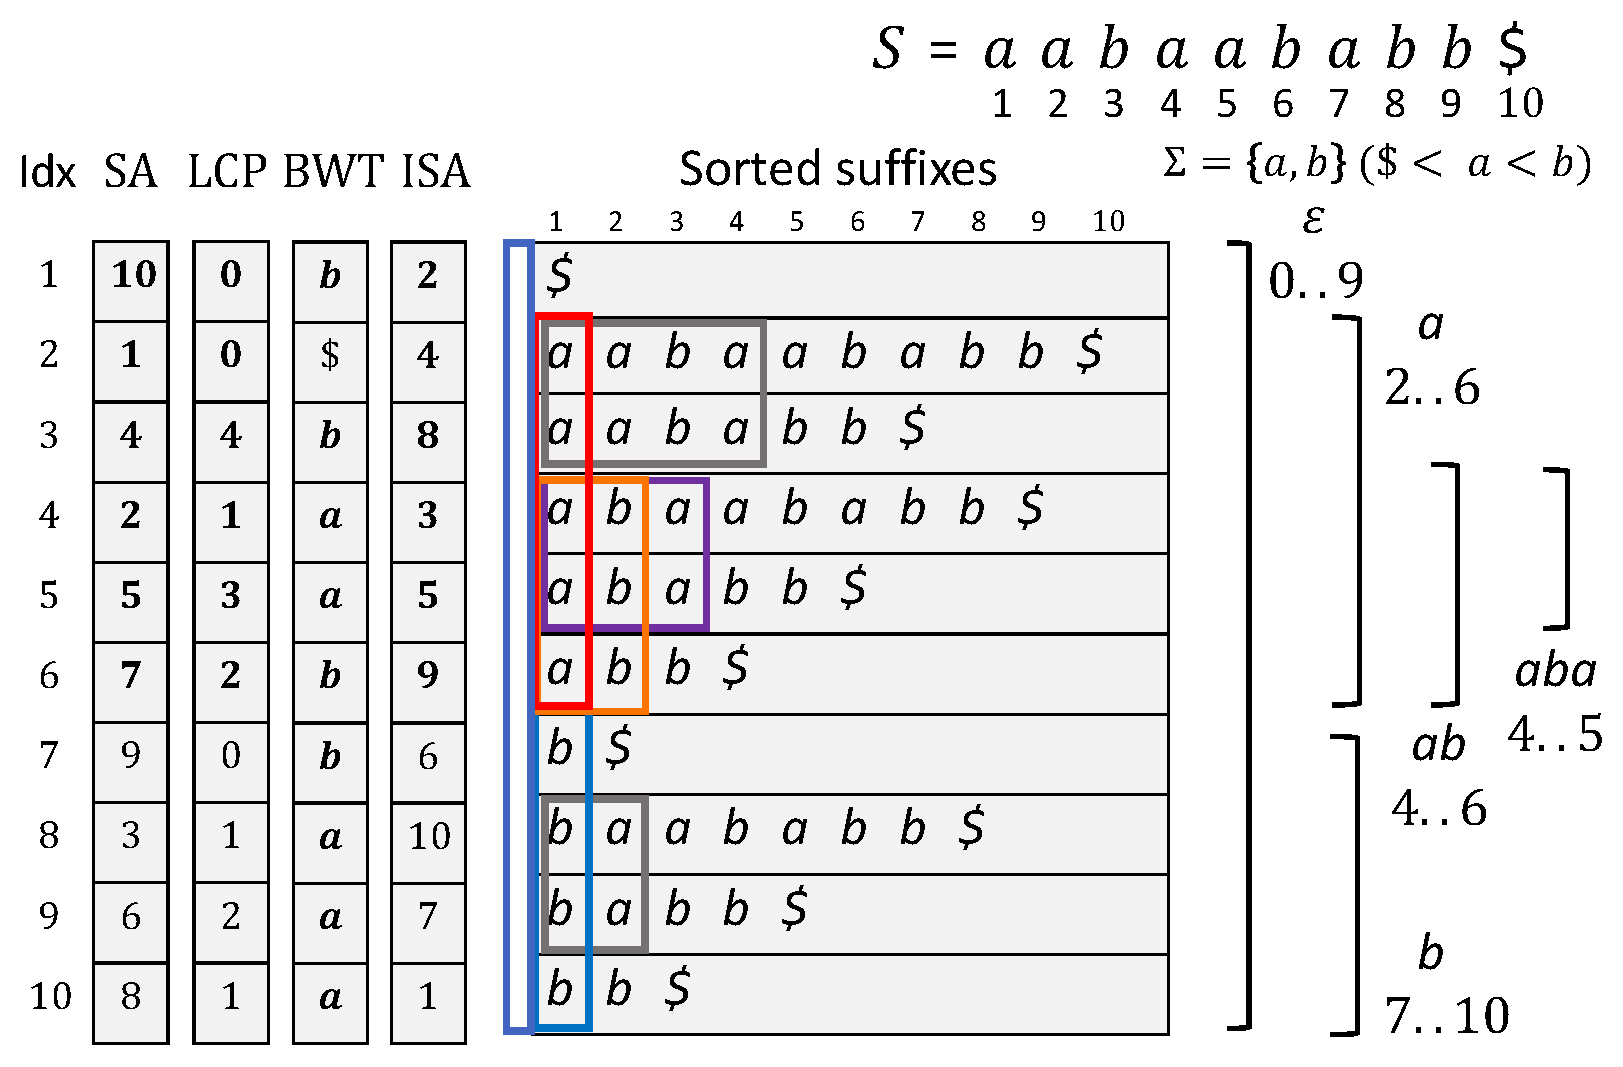
\includegraphics[width=0.60\textwidth]{fig/exp1/fig1.pdf}
%% \vspace{.5\baselineskip}
%% \caption{An example of minimal absent words of the string $S = \texttt{aabaababb}$. 
%% }\label{fig:example:maw}
%% \end{figure}
%% %%%%%%
%% %%%%%%%%%%%%%%%%%
%% \bgroup
%% {
%%   \setlength{\interspacetitleruled}{0pt}%
%%   \setlength{\algotitleheightrule}{0pt}%  
%%   \begin{algorithm}[h]
%%   %% \caption{Top-down MR-enumeration algorithm with \SA}\label{algo:maxrep:tdfw}
%%   \textbf{Procedure} \MRRec$(\tau_0 = ([L_0..R_0], \ell_0))$:\\
%%   %%\KwGiven{}
%%   %% \KwIn{The triple $\tau_0 = (L_0, R_0, \ell_0)$ for a right-branching substring $X$ of a string.}
%%   %% \KwOut{}
%%   \Begin{
%%       \textbf{output} $\tau_0$
%%       \Comment*{A maximal repeat is found}
%%       \For %(\CM{})
%%            {child $\tau = ([L..R], \ell)$ of the parent $([L_0..R_0], \ell_0)$}{
%%           \Comment{It is ensured that $R - L \ge 1$ and $\tau$ is right-branching}
%%           Decide if $\tau$ is left-branching by $\SA, \ISA$, and $S$ (\cref{lem:leftmaximal:character})\; 
%%           \If {$\tau$ is left-branching}{          
%%             \MRRec$(\tau)$\; 
%%           }
%%         }
%%   }
%%   \end{algorithm}
%% \egroup
%% %%%%%%%%%%%%%%%%%



%%% EOF
